% Ausgangslage (Ist-Analyse)

\section{Ausgangslage}
\label{sec:Ausgangslage}

\subsection{Anwendungsumfeld}
\label{subsec:Anwendungsumfeld}

%TODO
% Freistellen
\piccaption{Induktionsherd}
\parpic{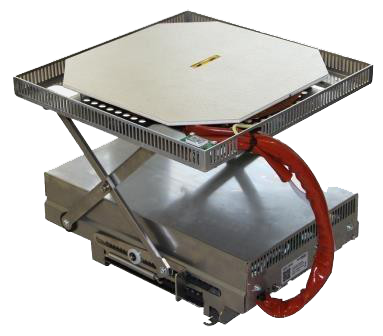
\includegraphics[scale=0.4]{analysis/res/einbaugeraete}}
Die Firma Fluxron AG mit Sitz in Amriswil TG bietet induktive Heiz- und Energiesysteme für Grossküchen an. Die Produktpalette besteht aus verschiedenen Induktionsherden und Thermostatsystemen. Diese haben jeweils ein Bluetoothmodul eingebaut, welches auf ein CANopen-basiertes Protokoll zur Kommunikation setzt. Die Module liefern neben den Geräteeinstellungen auch Fehlercodes und Sensormesswerte via Blootooth.
\picskip{0}
Fluxron verkauft diese Induktionsgeräte an Servicefirmen, welche diese dann beim Endkunden, z.B. einem Restaurant, einbauen und installieren. Dabei, aber auch bei Wartungsarbeiten, setzen die Servicefirmen die bestehende Android Applikation \enquote{FLX Tool} zur Diagnose und zur Konfiguration ein.

Neben den Servicefirmen, setzen auch die Mitarbeiter der Firma Fluxron die Androidapplikation bei internen Versuchen oder zur Ferndiagnose ein. Bei der Ferndiagnose wird eine Teamviewer-Verbindung auf das Smartphone oder den PC des Technikers aufgebaut. Über diese kann dann eine Diagnose mittels den Tools via Bluetooth erfolgen.

\subsection{Bestehende Android-Applikation - Fluxron Systemkonfigurator }
\label{subsec:Bestehende Smartphone-Applikation}
In Eigenentwicklung wurde bei Fluxron bereits eine einfache Android-Applikation entwickelt. Diese unterstützt bereits das Suchen von Geräten, sowie das Lesen und Schreiben von Parametern. Da diese App allerdings immer nur ein Gerät gleichzeitig bedienen kann und die Benutzerinteraktion daher sehr Zeitaufwändig ist, soll im Rahmen dieses Projektes eine neue, übersichtlichere Androidapplikation entstehen. In den nachfolgenden Abschnitten sind die Funktionen dieser Applikation aus funktioneller Sicht aufgelistet.

%TODO Screenshots

\subsubsection{Installation und Konfiguration}
\label{subsubsec:Installation und Konfiguration}
Die App kann ist öffentlich im Google Play Store erhältlich. Nach dem Download muss der Benutzer aber ein Kennwort eingeben, um Zugang zur App und den Gerätefunktionen zu erhalten.

\subsubsection{Verbindungsaufbau zu einem Gerät}
\label{subsubsec:Verbindungsaufbau zu einem Gerät}
Um eine Verbindung mit einem Gerät herzustellen, muss dieses zuerst über einen Suchlauf gefunden werden. Der Suchlauf zeigt alle momentan aktiven Geräte in einer Liste mit ihrer Device-ID an. In der Liste sind neben den aktiven Geräten auch alle Geräte aufgelistet, welche schon einmal mit der App verbunden waren.

Danach kann man sich mit einem Gerät aus der Liste verbinden um mit dem Gerät zu interagieren.

\subsubsection{Statusansicht}
\label{subsubsec:Statusansicht}
Wenn ein Gerät verbunden ist, kann der Benutzer über die entsprechende Schaltfläche zum Gerätetyp zu der Statusübersicht des Gerätes gelangen. Auf der Statusübersicht kann der Benutzer u.a. folgende Informationen auslesen:
\begin{itemize}
\item Statuscode
\item Temperatur des Kühlkörpers
\item Temperaturgradient
\item Pfannenerkennung
\item Soll- und Ist-Temperaturen der einzelnen Zonen
\item Leistungsaufnahme
\end{itemize}

\subsubsection{Setupansicht}
\label{subsubsec:Setupansicht}
Wenn ein Gerät verbunden ist, kann in der Setupansicht eine Liste aller Parameter des Gerätes ausgelesen werden. Der Benutzer kann Parameter anwählen, eine kurze Beschreibung dazu ansehen und deren Werte ändern.

\subsubsection{Historyansicht}
\label{subsubsec:Ansichten}
In der Historyansicht können Betriebszähler eingesehen. Dies beinhaltet Werte wie z.B. die Anzahl von "Power-On" Events oder Laufzeit des Gerätes.

Neben den Zähler kann ein Fehlerlog eingesehen werden, welches die letzten Zehn Fehlercodes beinhaltet. Dies kann zur Diagnose von Problemen sehr hilfreich sein.

\subsubsection{Einschränkungen der App}
\label{subsubsec:Einschränkungen der App}
\begin{itemize}
\item Es kann immer nur ein Gerät gleichzeitig verbunden sein
\item Für jede Verbindung ist ein erneuter Suchlauf nötig
\item Die Geräte sind nur mit der ID sichtbar, dies macht die Orientierung in einer Grossküche mit einem dutzend Geräten schwierig
\item Wenn ein nicht verbundenes Gerät eine Fehlermeldung absetzt, wird diese nicht empfangen
\item Typ der verbundenen Geräte wird zwar erkannt, die Benutzeroberfläche bietet aber immer noch alle Gerätetypen an
\end{itemize}

\subsection{Weitere bestehende Software}
\label{subsec:Weitere bestehende Software}
\subsubsection{FLX Access}
\label{subsubsec:FLX Access}
\piccaption{FLX Access}
\parpic{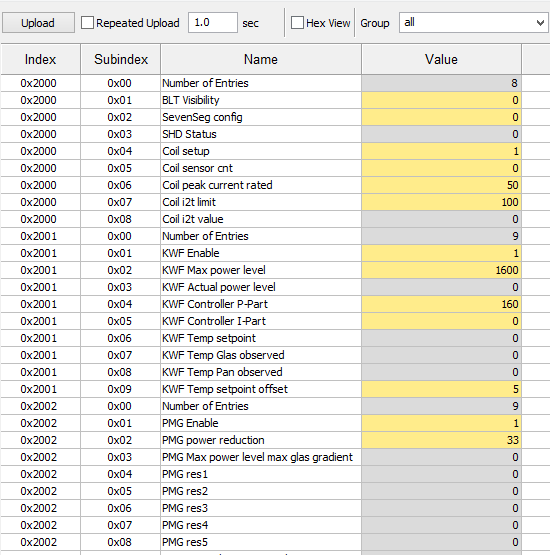
\includegraphics[scale=0.4]{analysis/res/flxaccess}}
Mit FLX Access stellt Fluxron ein Windows-Tool zum auslesen und setzen von gerätespezifischen Parametern bereit. Die Kommunikation erfolgt via Bluetooth. Zudem kann der Gerätestatus ausgelesen werden. 

Dieses System ist besonders für die Entwicklungsphase von Geräten gedacht.
\picskip{0}
\subsubsection{FLX Downloadtool}
\label{subsubsec:FLX Downloadtool}

\piccaption{FLX Access}
\parpic{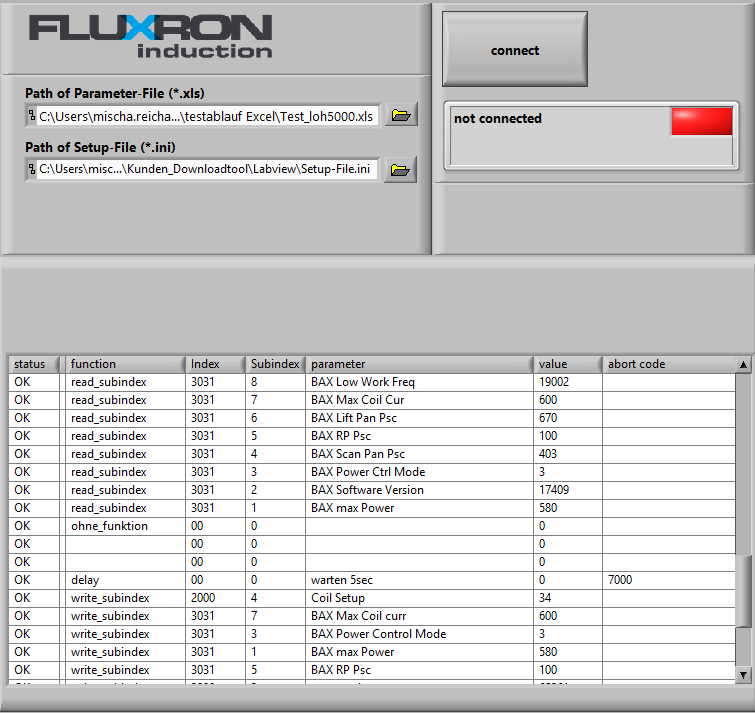
\includegraphics[scale=0.25]{analysis/res/flxdltool}}
Das FLX Downloadtool ermöglicht den Download der gesamten Konfiguration in eine Excel-Datei. In dieser können dan die Parameter eingestellt werden. Danach werden die Einstellungen über das Tool wieder auf das Gerät geladen.

Eingesetzt wird dieses Programm für das Schreiben von kundenspezifischen Parametern auf mehrere Geräte.
\picskip{0}